%************************************************
\chapter{Signal regions}
\label{ch:SR}
%************************************************

The signal region (SR) is a set of selections of events, such that the signal is rich and the background is small.
It is designed to discover the new particles, or set a limit on the masses of the hypothetical particles.
In the analysis, two signal regions are defined, SRjet1 and SRjet23.
Number of signal jets for SRjet1 is 1, while number of signal jets for SRjet23 is 2 or 3.
The details of the definition of these two signal regions will be described in section \ref{sec:signal_region_optimization}.

\section{Discriminant variables}
The discriminant variables are designed to define the signal regions.
The discriminant variables need to have the ability to distinguish the signal events from the background events, by applying a cut on the discriminant variable.
The following are the discriminant variables used in this analysis.
\begin{itemize}
\item $n_{\text{jets}}$: Number of signal jets:
\item $n_{\text{b-jets}}$: Number of $b$-jets.
\item $p_T^1$: Transverse momentum of the leading lepton.
\item $p_T^2$: Transverse momentum of the sub-leading lepton.
\item $\Delta \eta_{ll}$:
The difference in pseudorapidity between the two leptons.
\begin{equation}
\Delta \eta_{ll} = |\eta_{1} - \eta_{2}|
\end{equation}
\item $m_{ll}$:
It is the invariant mass of the two leptons (i.e. the invariant mass of the 4-momentum sum of the two leptons).
\begin{align}
(m_{ll})^2 = (p_1 + p_2)^2
\end{align}
\item $E_{T}^{\text{miss}}$:
The magnitude of the missing transverse momentum.
\begin{equation}
E_{T}^{\text{miss}} = |{\bf p}_T^{\text{miss}}|
\end{equation}
\item $m_T$:
It is designed to reconstruct the mass of the W-boson.
It is calculated by using the transverse momentum of the leading lepton and the missing transverse momentum, defined by equation \ref{equ:mT_def}.
By using the approximation $|{\bf p}_T^1| > 10$ GeV $\gg m_1$ (0.511 MeV or 106 MeV) and hence $E_T^1 = \sqrt{ (m_1)^2 + |{\bf p}_T^1|^2 } \approx |{\bf p}_T^1| $, it can be approximated by $m_T = \sqrt{2p_T^1 E_T^{\text{miss}}(1-\cos{\Delta\phi})}$, where $\Delta\phi$ is the azimuthal angle between the leading lepton and the missing transverse momentum.
\begin{align}
(m_T)^2 &= ( E_T^1 + E_T^{\text{miss}} )^2 - |{\bf p}_T^1 + {\bf p}_T^{\text{miss}}|^2 \label{equ:mT_def}\\
& \approx (|{\bf p}_T^1| + |{\bf p}_T^{\text{miss}}|)^2 - |{\bf p}_T^1 + {\bf p}_T^{\text{miss}}|^2 \\
&= (p_T^1 +  p_T^{\text{miss}})^2 - ({\bf p}_T^1 + {\bf p}_T^{\text{miss}}) \cdot ({\bf p}_T^1 + {\bf p}_T^{\text{miss}}) \\
&= (p_T^1)^2 + (p_T^{\text{miss}})^2 + 2 p_T^1 p_T^{\text{miss}}
 - (p_T^1)^2 - (p_T^{\text{miss}})^2 - 2 {\bf p}_T^1  \cdot {\bf p}_T^{\text{miss}} \\
&= 2 p_T^1 p_T^{\text{miss}} - 2 {\bf p}_T^1  \cdot {\bf p}_T^{\text{miss}} \\
&= 2 p_T^1 p_T^{\text{miss}} - 2 p_T^1 p_T^{\text{miss}} \cos{\Delta\phi} \\
&= 2 p_T^1 p_T^{\text{miss}} ( 1 - \cos{\Delta\phi} ) \\
m_T &= \sqrt{ 2 p_T^1 E_T^{\text{miss}} ( 1 - \cos{\Delta\phi} ) } \label{equ:mT_approx}
\end{align}
\item $m_{\text{eff}}$:
Effective mass is defined as the sum of the transverse momenta of the two leptons, signal jets and the missing transverse energy.
\begin{align}
m_{\text{eff}} = p_T^1 + p_T^2 + E_T^{\text{miss}} + \sum_{\text {signal jets}} p_T
\end{align}
\item $m_{lj}$ or $m_{ljj}$:
$m_{lj}$ is for the case that $n_{\text{jets}} = 1$ (i.e. SRjet1), while $m_{ljj}$ is for the case that $n_{\text{jets}} = 2$ or $3$ (i.e. SRjet23).
It attempts to reconstruct the mass of the Higgs boson.
It is defined as the invariant mass of the leading jet (i.e. the jet with the highest $p_T$) for SRjet1 or the di-jet system (i.e. the sum of the two leading jets) for SRjet23, and the closest lepton to the jet system, where the measure of distance is $\Delta R = \sqrt{(\Delta\phi)^2 + (\Delta\eta)^2}$.
The details of the definition are shown below.

The 4-momentum of the jet system is defined as
\begin{align}
p_{\text{jet-system}} =
\left\{
\begin{array}{ll}
p_{\text{jet1}} &\text{ for SRjet1}\\
p_{\text{jet1}} + p_{\text{jet2}} &\text{ for SRjet23}
\end{array} \right.
\end{align}

The 4-momentum of the closest lepton is defined as
\begin{align}
p_{\text{closest-lepton}} =
\left\{
\begin{array}{ll}
p_{\text{lepton1}} &\text{ if } \Delta R(p_{\text{lepton1}},p_{\text{jet-system}}) \leq \Delta R(p_{\text{lepton2}},p_{\text{jet-system}}) \\
p_{\text{lepton2}} &\text{ if } \Delta R(p_{\text{lepton1}},p_{\text{jet-system}}) > \Delta R(p_{\text{lepton2}},p_{\text{jet-system}})
\end{array} \right.
\end{align}

$m_{lj}$ or $m_{ljj}$ is defined as the invariant mass of the 4-momentum sum of the closest lepton and the jet system.
\begin{align}
(m_{lj(j)})^2 = (p_{\text{closest-lepton}} + p_{\text{jet-system}})^2
\end{align}

\item $m_{T2}$:
The ``stransverse mass'' ($m_{T2}$) is designed to set a lower bound on the masses of the unseen pair of charginos $\tilde{\chi}_1^\pm$ and neutralinos $\tilde{\chi}_2^0$.
One side is for charginos $\tilde{\chi}_1^\pm$ and another side is for neutralinos $\tilde{\chi}_2^0$, as shown in figure \ref{fig:signal_feynman}.
They are both assumed to decay into one lepton that can be detected, and into neutralinos $\tilde{\chi}_1^0$ and neutrino that cannot be detected and hence they contribute to the missing transverse momentum.
The calculation of $m_{T2}$ uses the transverse momentum of the two leptons (i.e. ${\bf p}_T^1$ and ${\bf p}_T^2$) and the missing transverse momentum ${\bf p}_T^{\text{miss}}$ as the inputs.
It is defined by finding the minimum value over all possible transverse vectors ${\bf q}_T$, which is the trial missing transverse momentum on one side \cite{MT2}.
\begin{equation}
m_{T2} = \min_{{\bf q}_T} \Bigg[ \max \bigg( m_T( {\bf p}_T^1, {\bf q}_T ), m_T( {\bf p}_T^2, {\bf p}_T^{\text{miss}} - {\bf q}_T ) \bigg) \Bigg]
\end{equation}
Similar to equation \ref{equ:mT_approx}, the transverse mass of two transverse momenta $m_T( {\bf p}_T, {\bf q}_T )$ is defined as follows.
\begin{equation}
m_T( {\bf p}_T, {\bf q}_T ) = \sqrt{ 2 p_T q_T ( 1 - \cos{\Delta\phi} ) }
\end{equation}
where $\Delta\phi$ is the azimuthal angle between the two transverse momenta.
\end{itemize}

\section{Signal region optimization}
\label{sec:signal_region_optimization}
This section describes how the signal region is found and optimizied.
The goal of the optimization is to increase the number of signal events $N_s$ and decrease the number of background event $N_b$.
This study was done, before we look at the real data, and hence the MC samples were used for signal and background.
The signal significance Z for large $N_s$ and $N_b$ is defined by
\begin{equation}
Z = \frac{N_s}{\sqrt{N_b + N_s}}
\label{equ:simple_significance}
\end{equation}
It measures how well the signal region is.
The process of the signal region optimization is to increase the signal significance Z.
The signal significance Z can be interpreted as the variable $z = \frac{x-\mu}{\sigma}$ in the standard normal distribution.
The corresponding p-value can be interpreted as the probability that the excess in the number of signal events from the background event is just due to the statistical fluctuation.
By changing the cuts on different discriminant variables, the maximum signal significance can be obtained, and the corresponding optimal cuts are the definition of the signal region.

Equation \ref{equ:simple_significance} is only valid for large $N_s$ and $N_b$.
Because $N_s$ and $N_b$ are often small, another sophisticated formula for the signal significance was used.
Also, the systematic error and statistical error of $N_b$ need to be taken account.
A fixed systematic error 25\% is used, and the total relative error $\sigma_b$ is the sum of systematic and statistical error in quadrature.
\begin{equation}
\sigma_b = \sqrt{(25\%)^2 + (\frac{\Delta N_b}{N_b})^2}
\end{equation}
where $\Delta N_b$ is the statistical error of $N_b$.
The signal significance is calculated by using the function \texttt{NumberCountingUtils::BinomialExpZ} provided in \texttt{RooStats}.
\begin{equation}
Z = \text{BinomialExpZ}(N_s,N_b,\sigma_b)
\label{equ:significance_def}
\end{equation}
This method basically calculates the signal significance Z with the corresponding p-value and probability for the following case.
A series of Bernoulli experiments is conducted with the number of trials $n = N_b + N_s + \frac{1}{\sigma_b ^2}$ and the probability of success of each trial $p = 1/(1 + 1/(N_b \sigma_b ^2))$ \cite{2-leptons-long}.
The corresponding p-value is the probability that the number of success is at least $N_b + N_s$.
The connection between these Bernoulli experiments and our analysis will not be explained here, but what is important is that the signal significance Z calculated by the equation \ref{equ:significance_def} is an approximation to our analysis. It is useful because it has the following properties.
\begin{itemize}
\item It is a continuous function. $N_b$ and $N_s$ can be non-integer. (cf. Poisson distribution)
\item It is a smooth function. It is convenient for finding the maximum value.
\item For large $N_b$ and $N_s$, it reduces to equation \ref{equ:simple_significance}.
\item It is fast to compute.
\end{itemize}
By using the equation \ref{equ:significance_def}, an approximately optimal signal region can be found.

\subsection{Pre-selection}
\label{sec:SR_pre-selection}
Before the optimization, the following pre-selections are applied, on top of the selections in section \ref{event_cleaning}.
\begin{itemize}
\item \textbf{Exactly 2 signal leptons} The events which have exactly 2 signal leptons are selected. This means that the two leptons must be signal leptons.
\item \textbf{Same sign} The electric charges of the two leptons have the same sign. This is what we are looking for, described in section \ref{sec:Wh_signal}.
\item \textbf{B-jet veto} To suppress the top background, the number of b-jets is 0.
\item \textbf{Number of jet} Similar to the Run 1 analysis, two signal regions are defined according to the number of signal jets. One signal region has 1 signal jet, called ``SRjet1'', and another has 2 or 3 signal jets, called ``SRjet23''.
\end{itemize}

\subsection{Samples}
As mentioned before, MC samples were used for estimating the expected $N_s$ and $N_b$ in the process of optimization.
For signal, the mass point ($m_{\tilde{\chi}_1^\pm , \tilde{\chi}_2^0}$,$m_{\tilde{\chi}_1^0}$) = (225,75) was used for SRjet1, while the mass point ($m_{\tilde{\chi}_1^\pm , \tilde{\chi}_2^0}$,$m_{\tilde{\chi}_1^0}$) = (187.5,37.5) was used for SRjet23.
For the background, MC samples were used for diboson (WZ, WW and ZZ), ttV and rare processes (triboson, multitop and Higgs).
The fake lepton background estimated by the matrix method in section \ref{sec:fake_background} was used, instead of using the corresponding MC samples, because the fake lepton background are the major background and the corresponding MC sample is not reliable.
The charge flip background estimated in section \ref{sec:charge_flip_background} was also used.
The plots after the pre-selection in section \ref{sec:SR_pre-selection}, but before the optimization, are shown in figures \ref{fig:SRjet1_pre-selection} and \ref{fig:SRjet23_pre-selection}.

\begin{figure}[htpb]
\centering
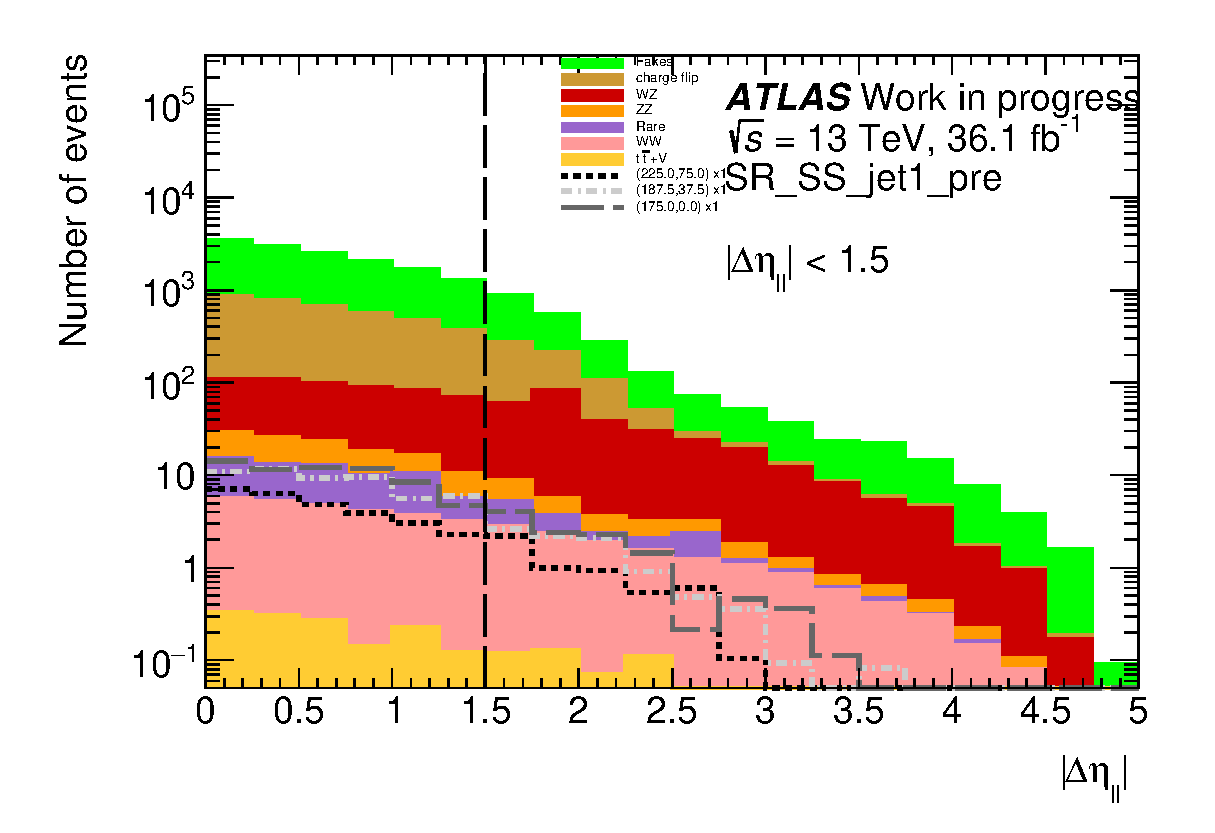
\includegraphics[width=0.45\linewidth]{data/plot/plot_SR/dEta_SR_SS_jet1_pre}
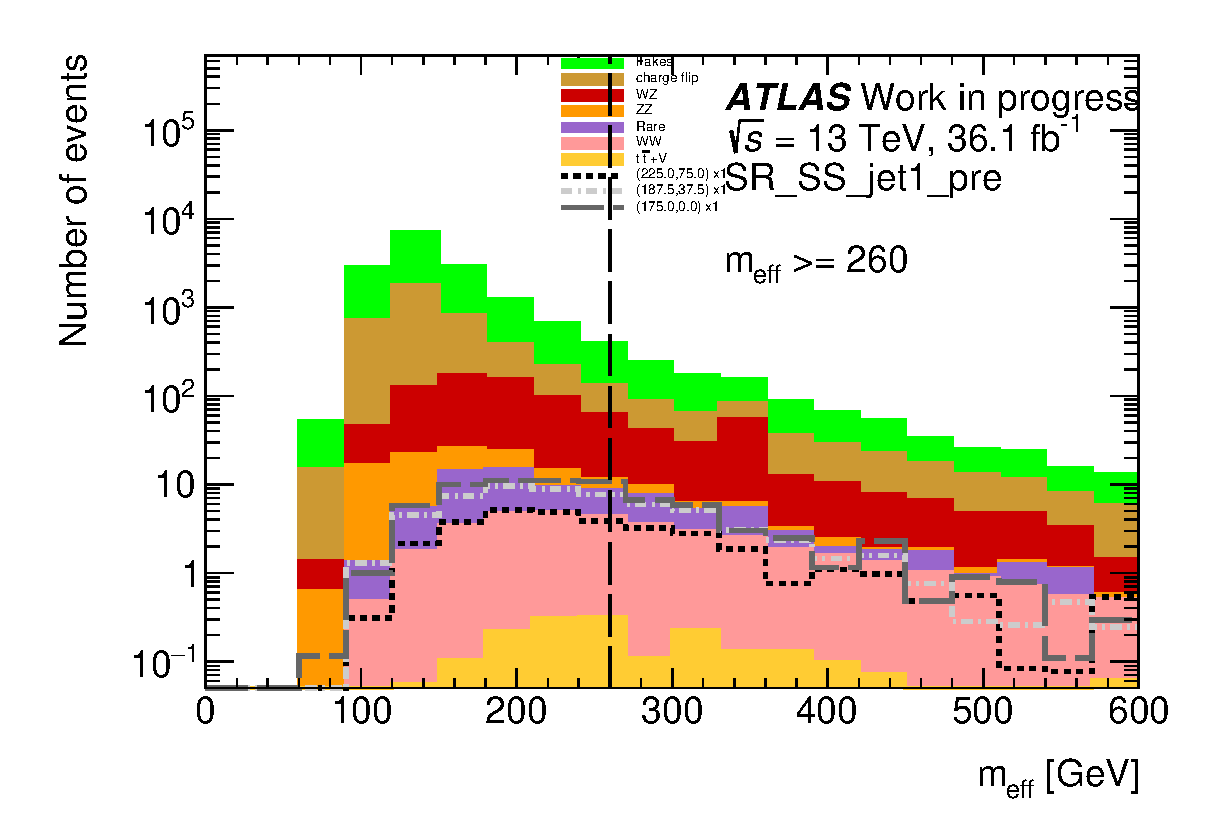
\includegraphics[width=0.45\linewidth]{data/plot/plot_SR/meff_SR_SS_jet1_pre}\\
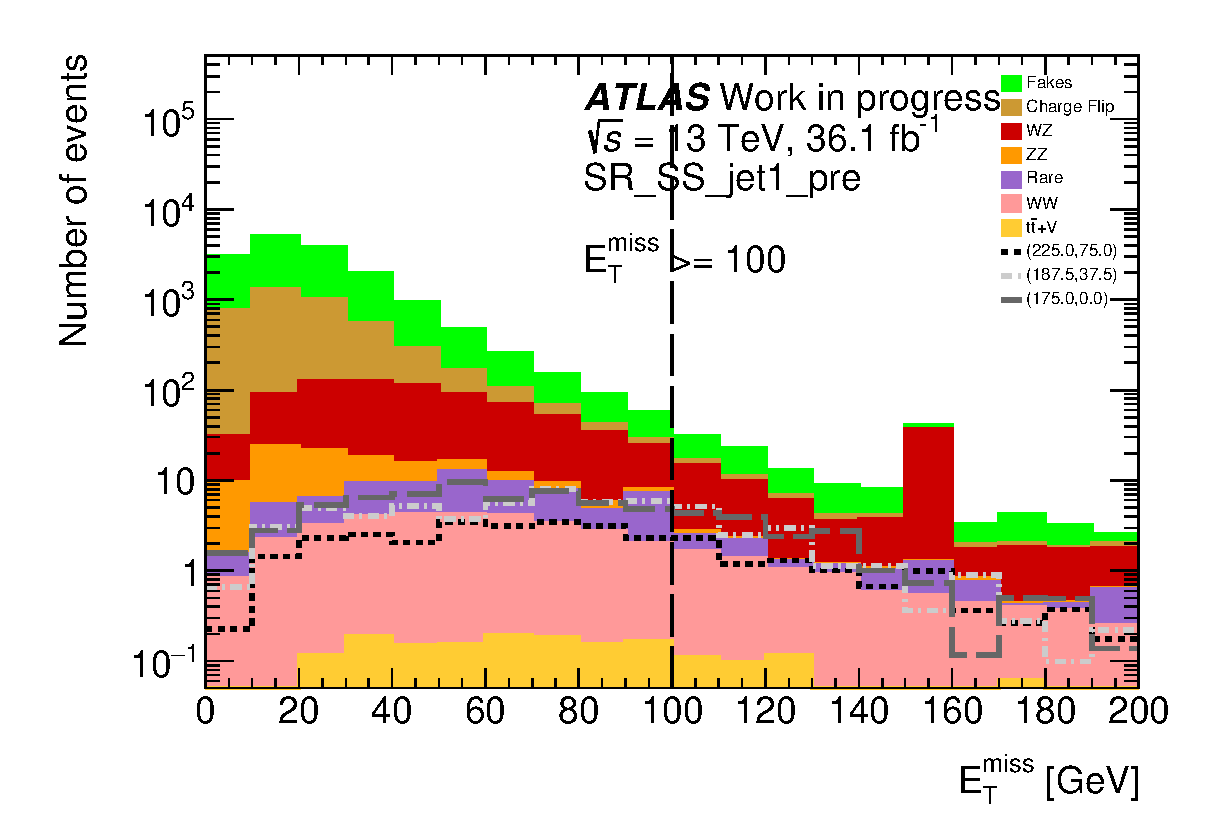
\includegraphics[width=0.45\linewidth]{data/plot/plot_SR/MET_SR_SS_jet1_pre}
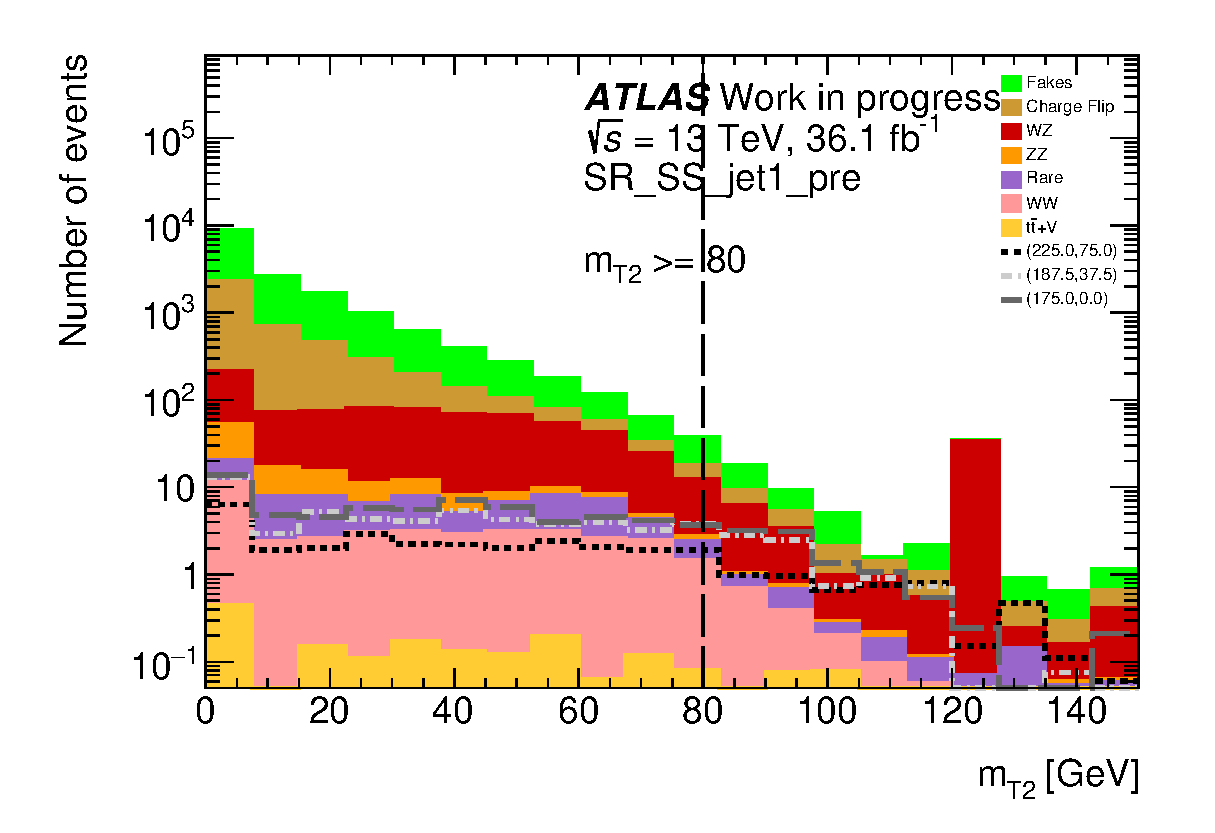
\includegraphics[width=0.45\linewidth]{data/plot/plot_SR/mTtwo_SR_SS_jet1_pre}\\
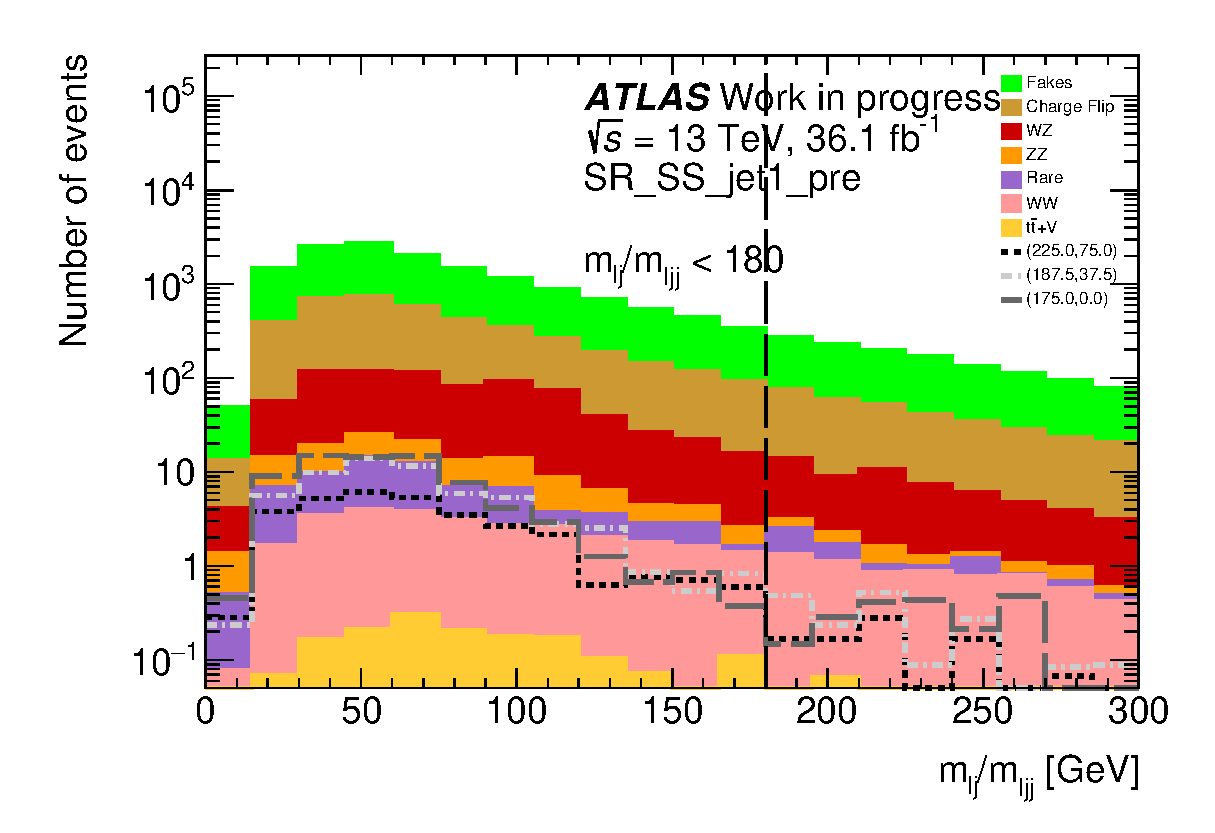
\includegraphics[width=0.45\linewidth]{data/plot/plot_SR/mlj_SR_SS_jet1_pre}
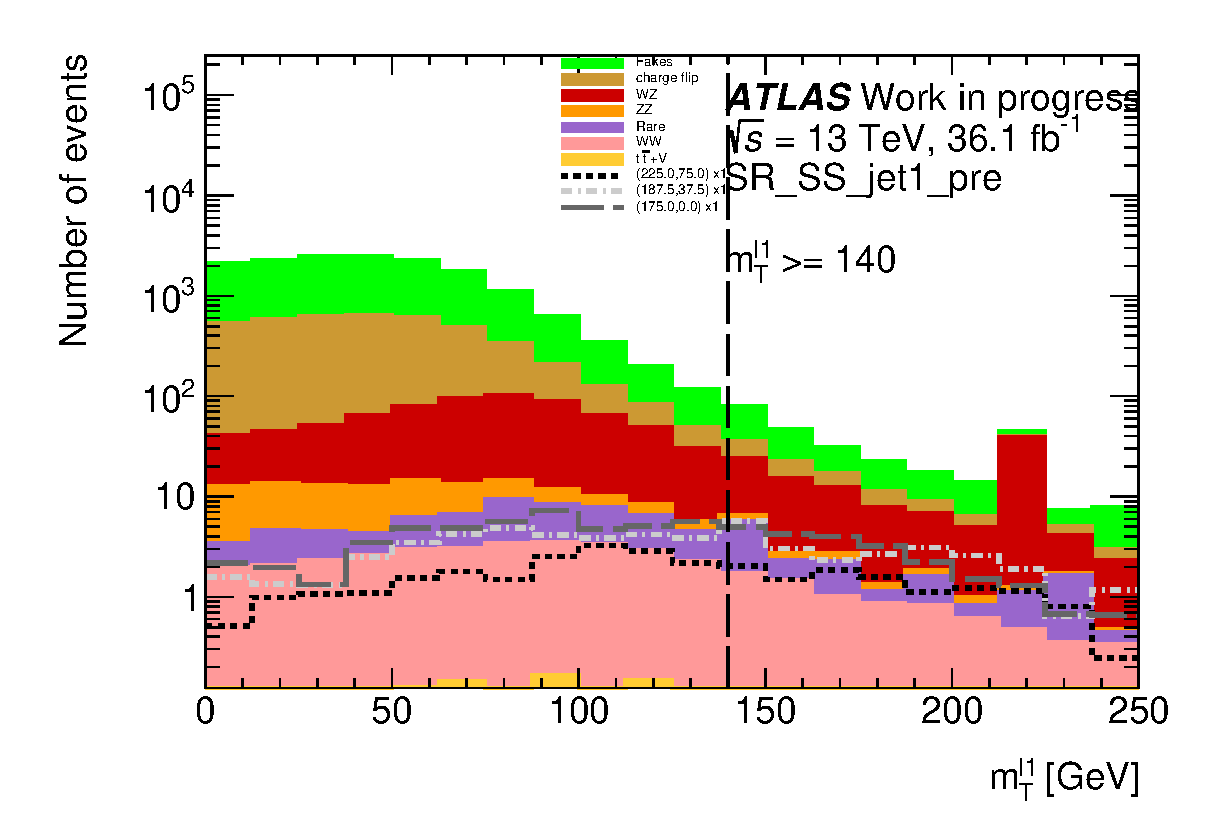
\includegraphics[width=0.45\linewidth]{data/plot/plot_SR/mt1_SR_SS_jet1_pre}\\
\caption{Distribution of the kinematic variables used for the optimization in SRjet1. The pre-selection has been applied.}
\label{fig:SRjet1_pre-selection}
\end{figure}

\begin{figure}[htpb]
\centering
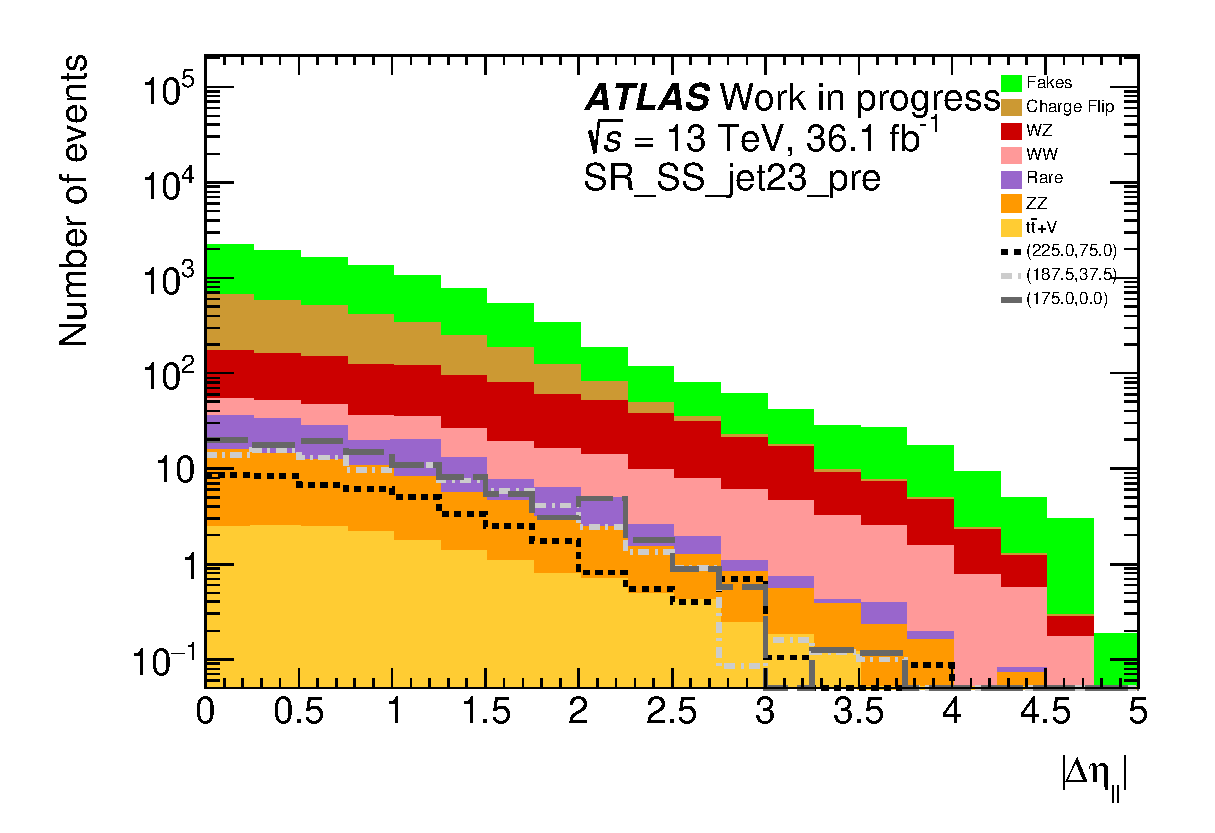
\includegraphics[width=0.45\linewidth]{data/plot/plot_SR/dEta_SR_SS_jet23_pre}
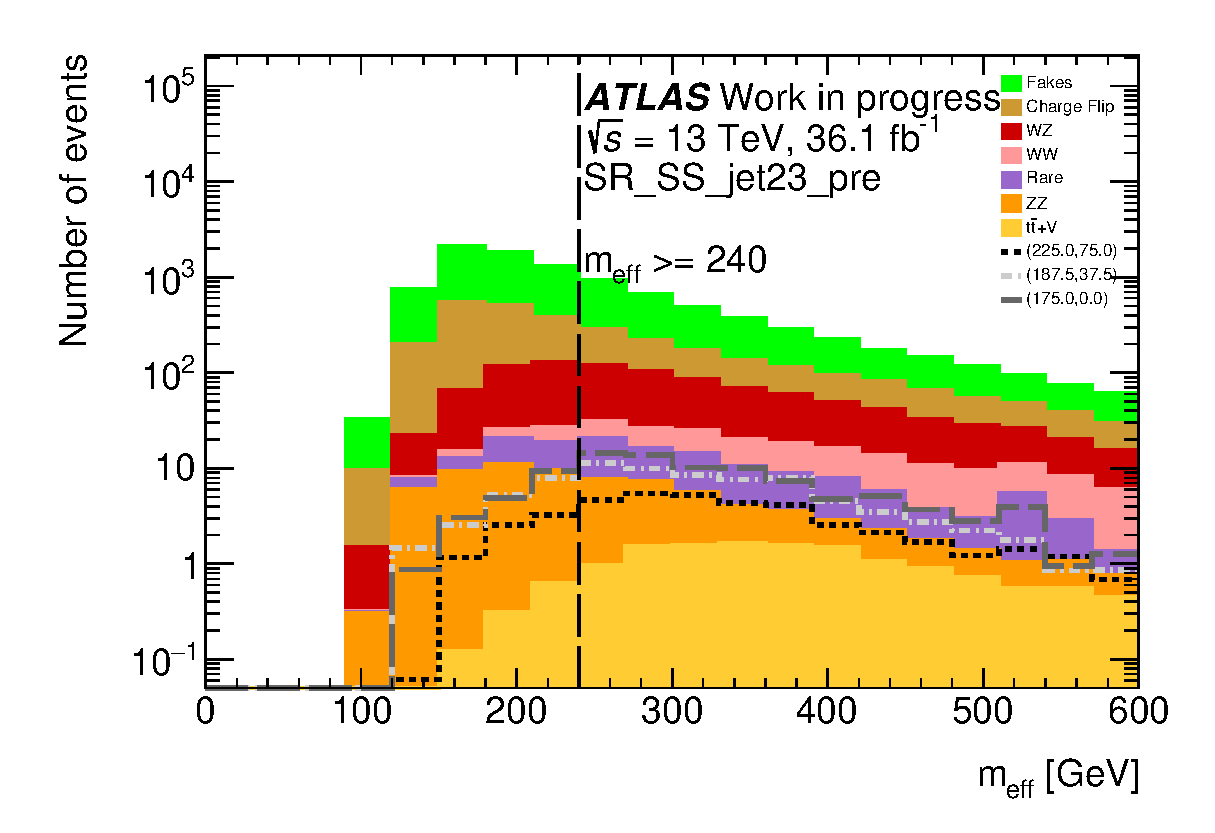
\includegraphics[width=0.45\linewidth]{data/plot/plot_SR/meff_SR_SS_jet23_pre}\\
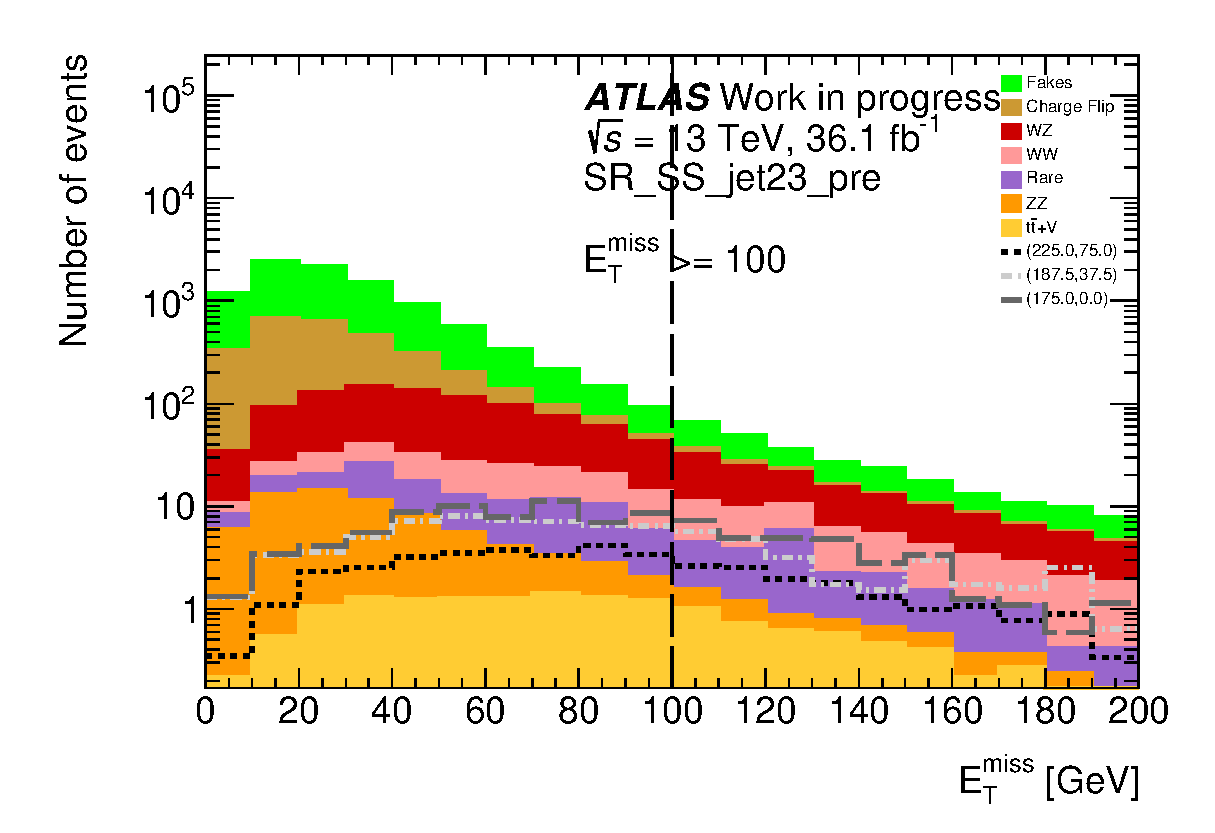
\includegraphics[width=0.45\linewidth]{data/plot/plot_SR/MET_SR_SS_jet23_pre}
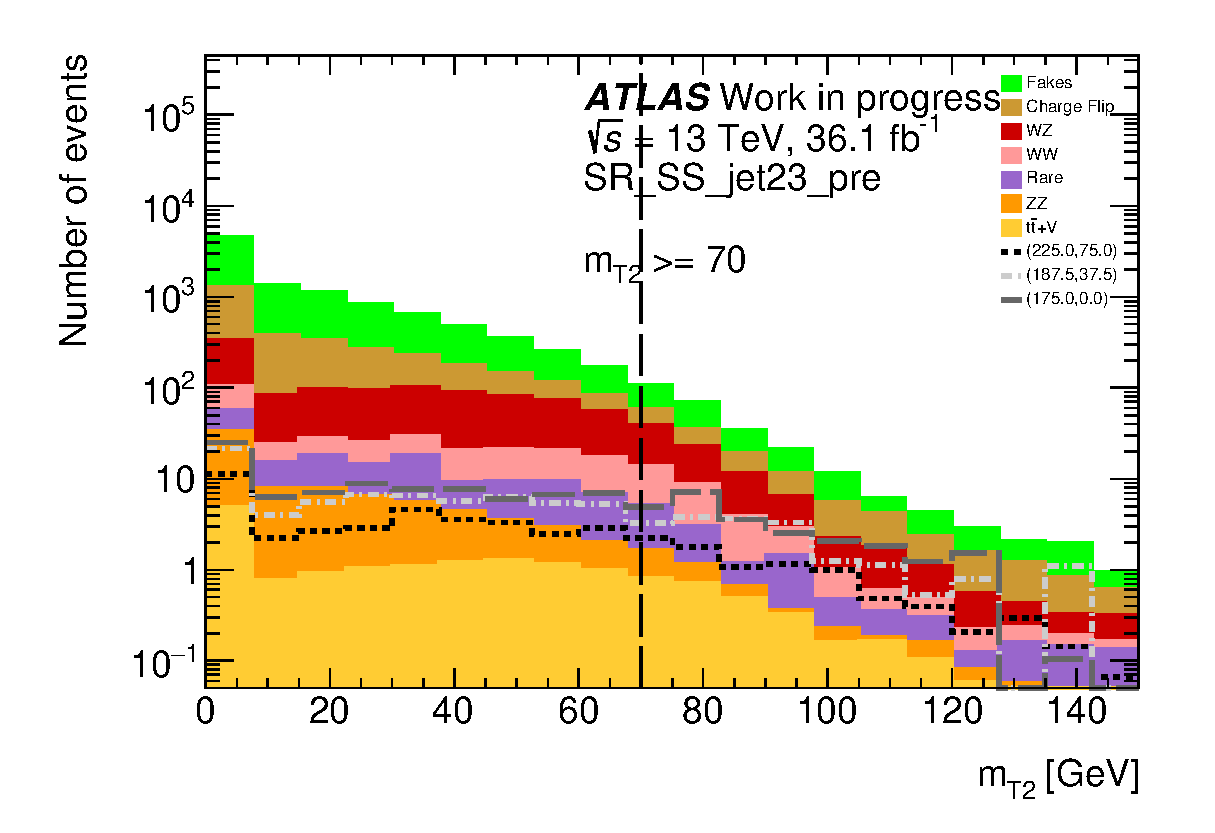
\includegraphics[width=0.45\linewidth]{data/plot/plot_SR/mTtwo_SR_SS_jet23_pre}\\
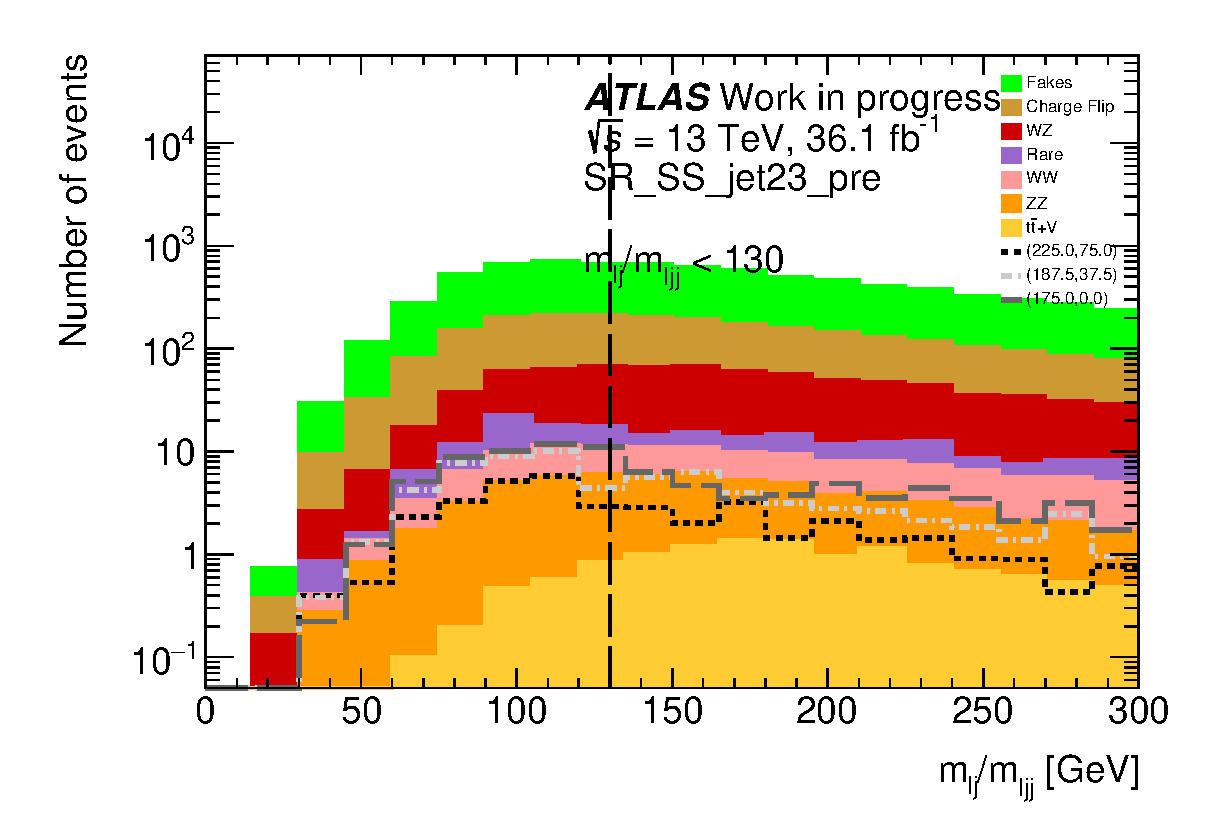
\includegraphics[width=0.45\linewidth]{data/plot/plot_SR/mlj_SR_SS_jet23_pre}
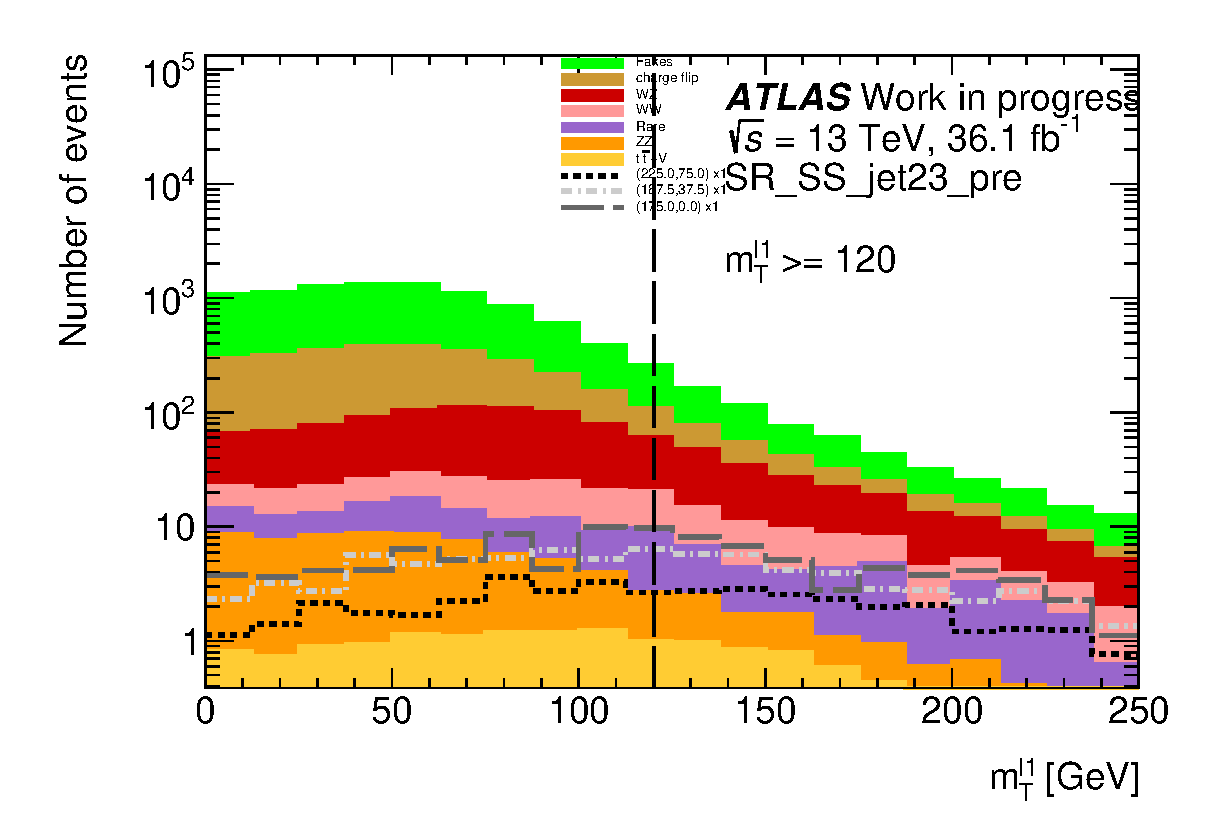
\includegraphics[width=0.45\linewidth]{data/plot/plot_SR/mt1_SR_SS_jet23_pre}\\
\caption{Distribution of the kinematic variables used for the optimization in SRjet23. The pre-selection has been applied.}
\label{fig:SRjet23_pre-selection}
\end{figure}

\subsection{Running for optimization}
Some constraints were applied during the process of optimization, in order to have enough statistics to have reliable estimation of $N_s$ and $N_b$.
\begin{itemize}
\item The yields (i.e. the sum of weighted events) for each process of background need to be positive, to have a reasonable and stable modelling of the background shape.
Also, the HistFitter requires the background need to have positive yields.
\item The diboson and ttV background have at least 10 unweighted events respectively, to have a reliable estimation for the main background processes from prompt leptons (i.e. not fake leptons).
\item For $E_T^{\text{miss}}$, $m_T$, $m_{\text{eff}}$ and $m_{T2}$, only lower cuts are applied.
\item For $\Delta \eta_{ll}$ and $m_{lj(j)}$, only upper cuts are applied.
\end{itemize}

The list of variables used is shown in the table \ref{tab:variables_optimization}.

\begin{table}[htbp]
\centering
\begin{tabular}{|c|c|}
\hline
Variable & direction of cut \\
\hline
\hline
$\Delta \eta_{ll}$ & upper cut \\
\hline
$E_T^{\text{miss}}$ & lower cut \\
\hline
$m_T$ & lower cut \\
\hline
$m_{\text{eff}}$ & lower cut \\
\hline
$m_{lj(j)}$ & upper cut \\
\hline
$m_{T2}$ & lower cut \\
\hline
\end{tabular}
\caption{Kinematic variables used in the optimization.}
\label{tab:variables_optimization}
\end{table}

\subsection{Results for optimization}
The final results for the definitions of the two signal regions are shown in table \ref{tab:SR_Def}.
The yields for different background and signal processes are shown in table \ref{tab:SRjet1_yields} and \ref{tab:SRjet23_yields}.
The N-1 plots for the discriminant variables are shown in figures \ref{fig:SRjet1_N1} and \ref{fig:SRjet23_N1}.
The N-1 plot means that all other SR selections are applied, except the selection for that variable.

\begin{table}[htpb]
\centering
\begin{tabular}{|c|c|c|}
\hline
Variable &  SRjet1 & SRjet23 \\ \hline
$\Delta\eta_{ll}$ & $\leq 1.5$ &  -- \\
$E_T^{\text{miss}}$ &  $\geq 100 $ GeV  & $\geq 100$ GeV\\
$m_T$ & $\geq 140$ GeV & $\geq 120$ GeV \\
$m_{\text{eff}}$ & $\geq 260$ GeV &  $\geq 240$ GeV\\
$m_{lj(j)}$ & $< 180$ GeV &  $< 130$ GeV\\
$m_{T2}$ & $\geq 80$ GeV&  $\geq 70$ GeV \\
\hline
\end{tabular}
\caption{Final SR definitions}
\label{tab:SR_Def}
\end{table}

\begin{table}[htpb]
\centering
\begin{tabular}{|c|c|c|}
\hline
& Number of events & Significance \\
\hline
\hline
Fakes & $3.295\pm0.819$ (24) & \\
\hline
WZ & $2.176\pm0.398$ (257) & \\
\hline
Charge Flip & $0.472\pm0.053$ (265) & \\
\hline
Rare & $0.444\pm0.111$ (56) & \\
\hline
WW & $0.166\pm0.023$ (67) & \\
\hline
$t\bar{t}+V$ & $0.125\pm0.046$ (36) & \\
\hline
ZZ & $0.055\pm0.028$ (31) & \\
\hline
\hline
Total BG & $6.733\pm0.921$ (736) & \\
\hline
\hline
(225.0,75.0) & $3.33\pm0.60$ (60) &$ \bf 0.74$\\
\hline
(187.5,37.5) & $3.77\pm0.95$ (31) &$0.86$\\
\hline
(175.0,0.0) & $4.29\pm0.73$ (36) &$0.98$\\
\hline
\end{tabular}
\caption{The yields in SRjet1. The unweighed event are also shown in parentheses.}
\label{tab:SRjet1_yields}
\end{table}

\begin{table}[htpb]
\centering
\begin{tabular}{|c|c|c|}
\hline
& Number of events & Significance \\
\hline
\hline
WZ & $1.849\pm0.273$ (319) & \\
\hline
Fakes & $1.765\pm0.709$ (20) & \\
\hline
Rare & $0.731\pm0.195$ (48) & \\
\hline
WW & $0.514\pm0.037$ (235) & \\
\hline
Charge Flip & $0.267\pm0.029$ (274) & \\
\hline
$t\bar{t}+V$ & $0.142\pm0.031$ (67) & \\
\hline
ZZ & $0.067\pm0.025$ (24) & \\
\hline
\hline
Total BG & $5.335\pm0.787$ (987) & \\
\hline
\hline
(225.0,75.0) & $2.35\pm0.34$ (58) &$0.57$\\
\hline
(187.5,37.5) & $4.72\pm0.74$ (47) &$\bf 1.26$\\
\hline
(175.0,0.0) & $8.60\pm1.51$ (58) &$2.24$\\
\hline
\end{tabular}
\caption{The yields in SRjet23. The unweighed event are also shown in parentheses.}
\label{tab:SRjet23_yields}
\end{table}

\begin{figure}[htpb]
\centering
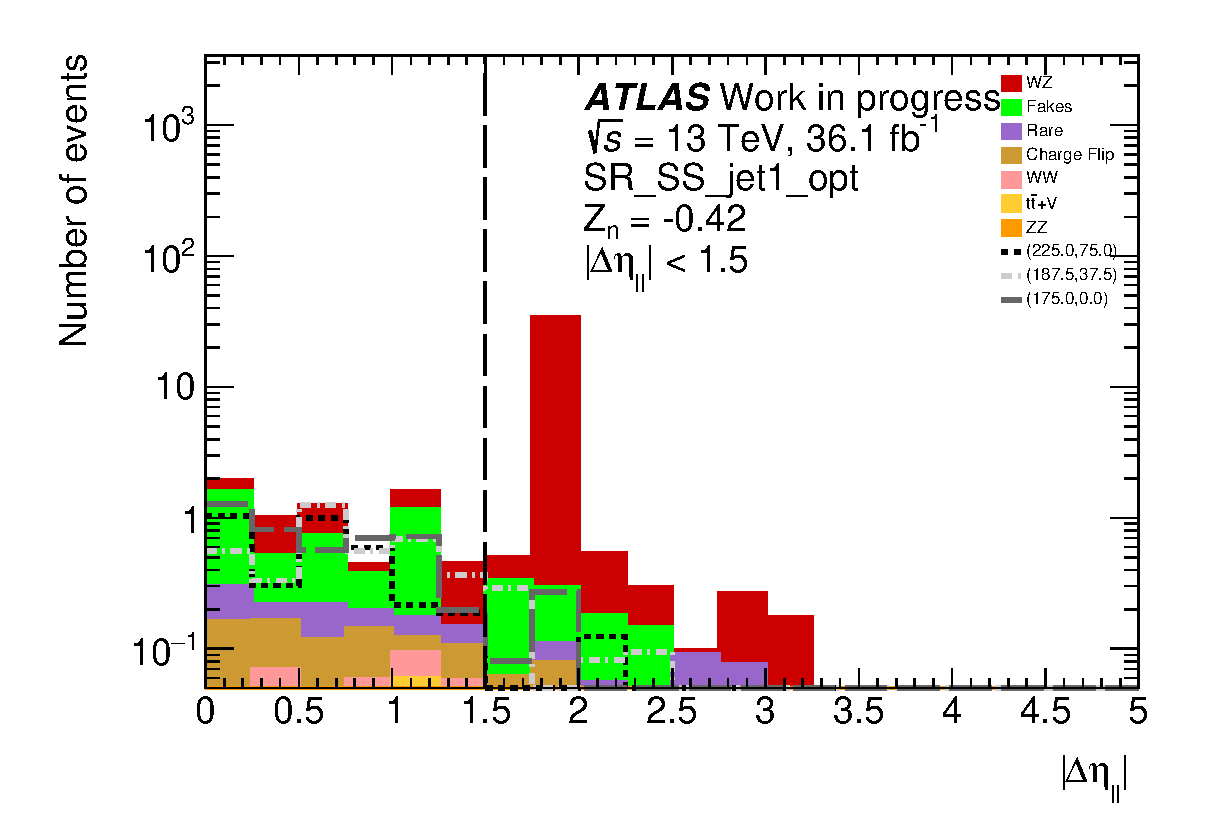
\includegraphics[width=0.45\linewidth]{data/plot/plot_SR/dEta_SR_SS_jet1_opt_0}
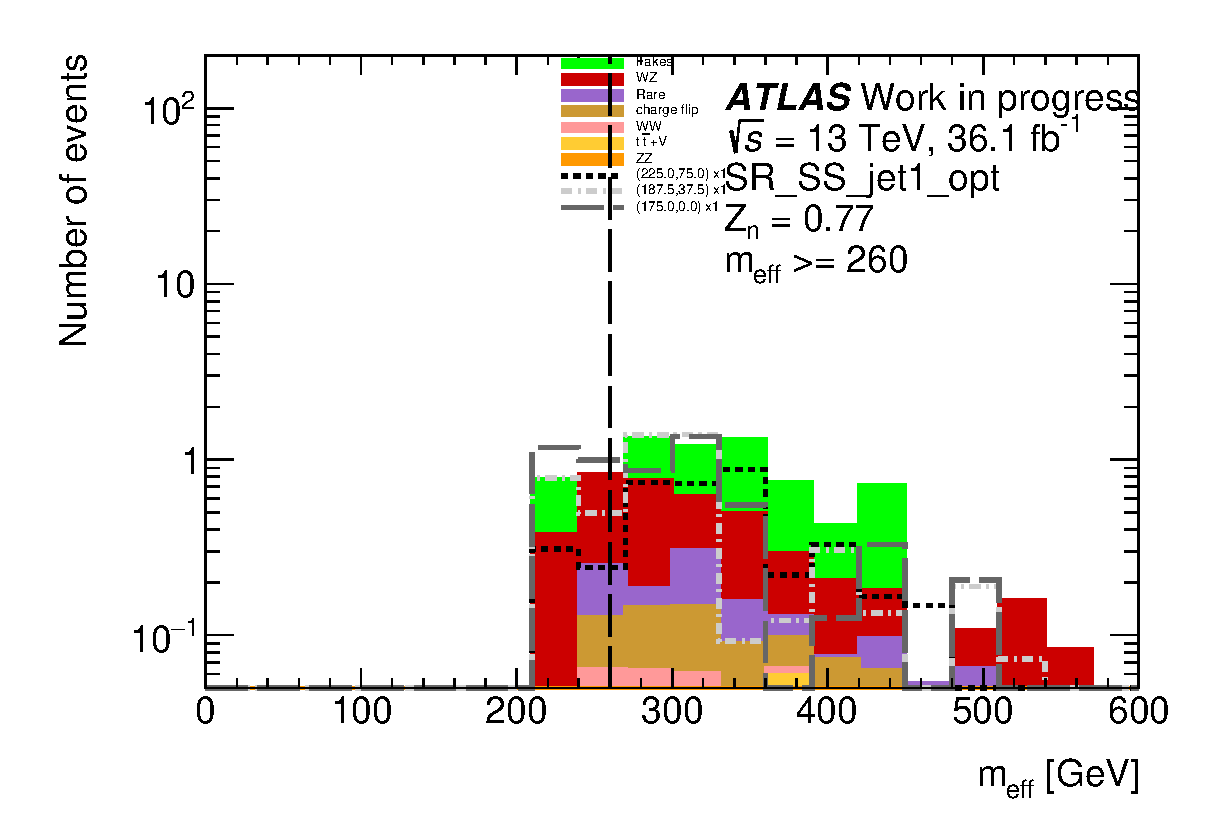
\includegraphics[width=0.45\linewidth]{data/plot/plot_SR/meff_SR_SS_jet1_opt_0}\\
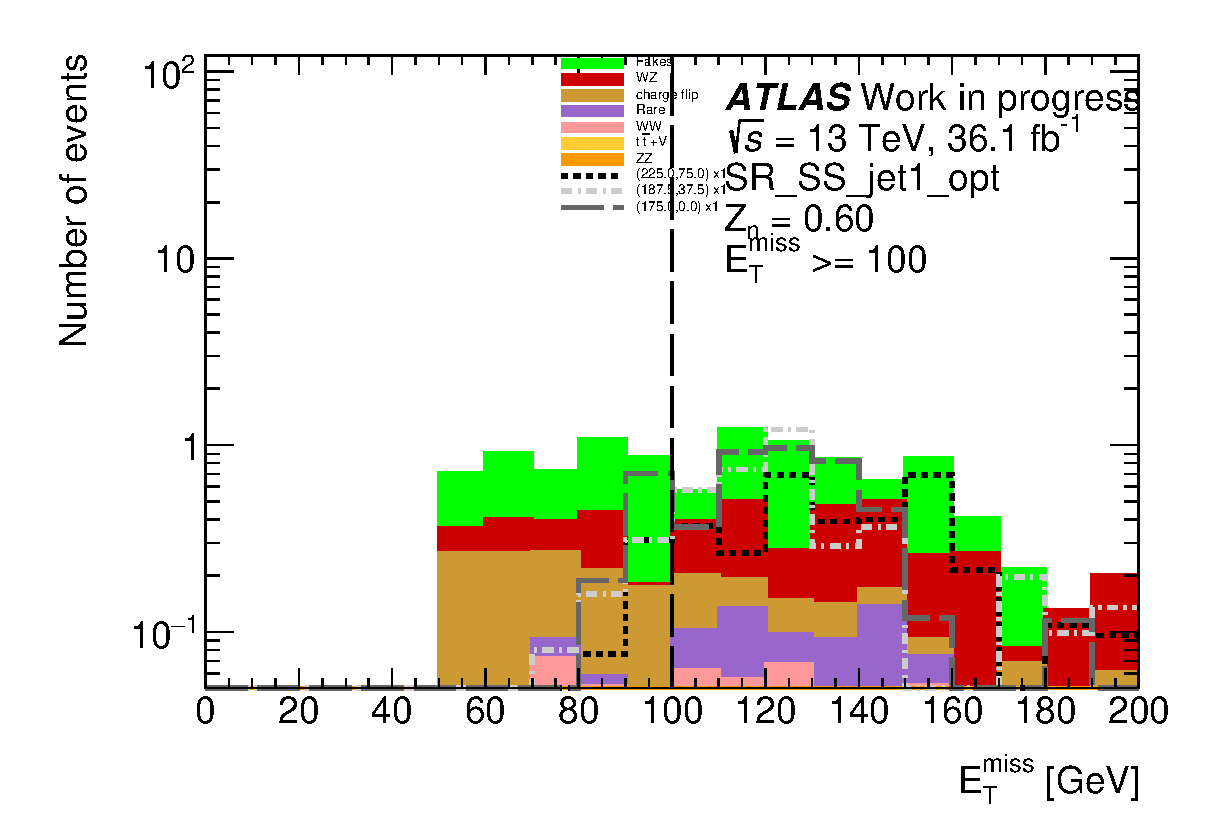
\includegraphics[width=0.45\linewidth]{data/plot/plot_SR/MET_SR_SS_jet1_opt_0}
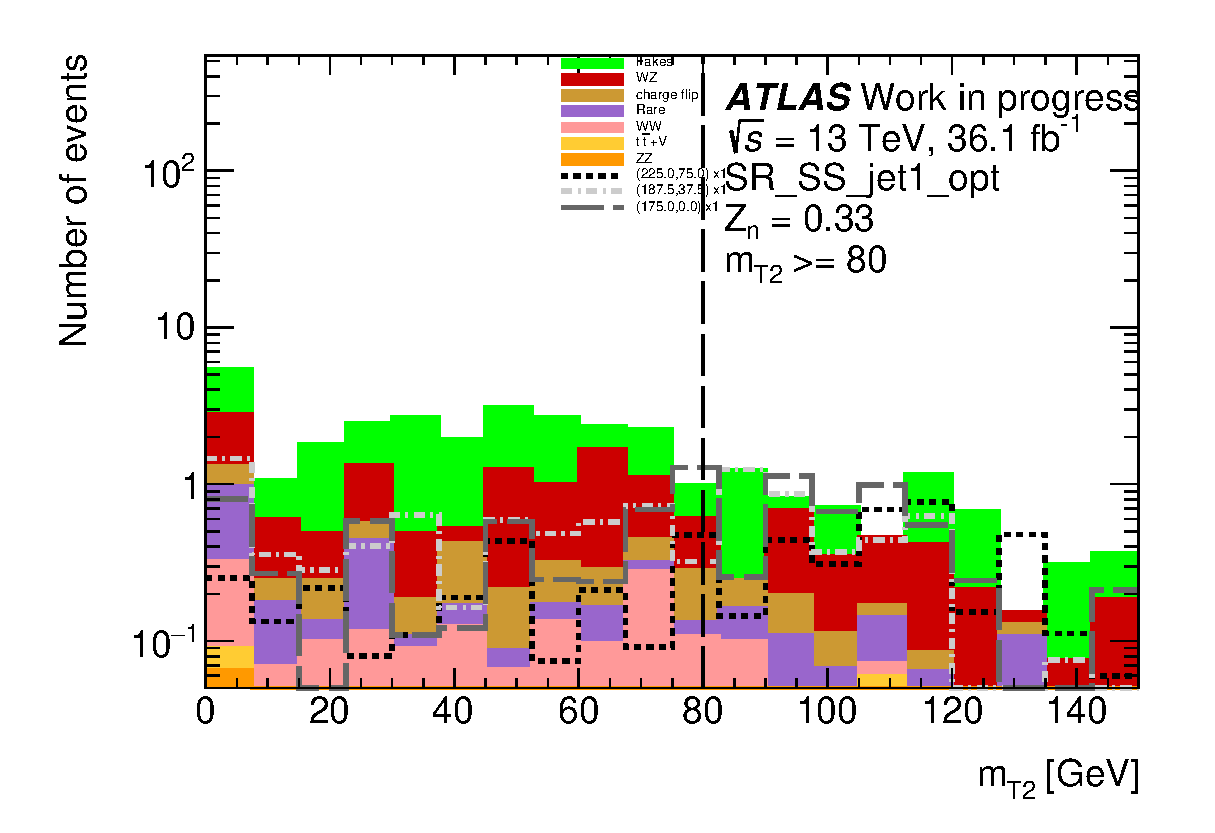
\includegraphics[width=0.45\linewidth]{data/plot/plot_SR/mTtwo_SR_SS_jet1_opt_0}\\
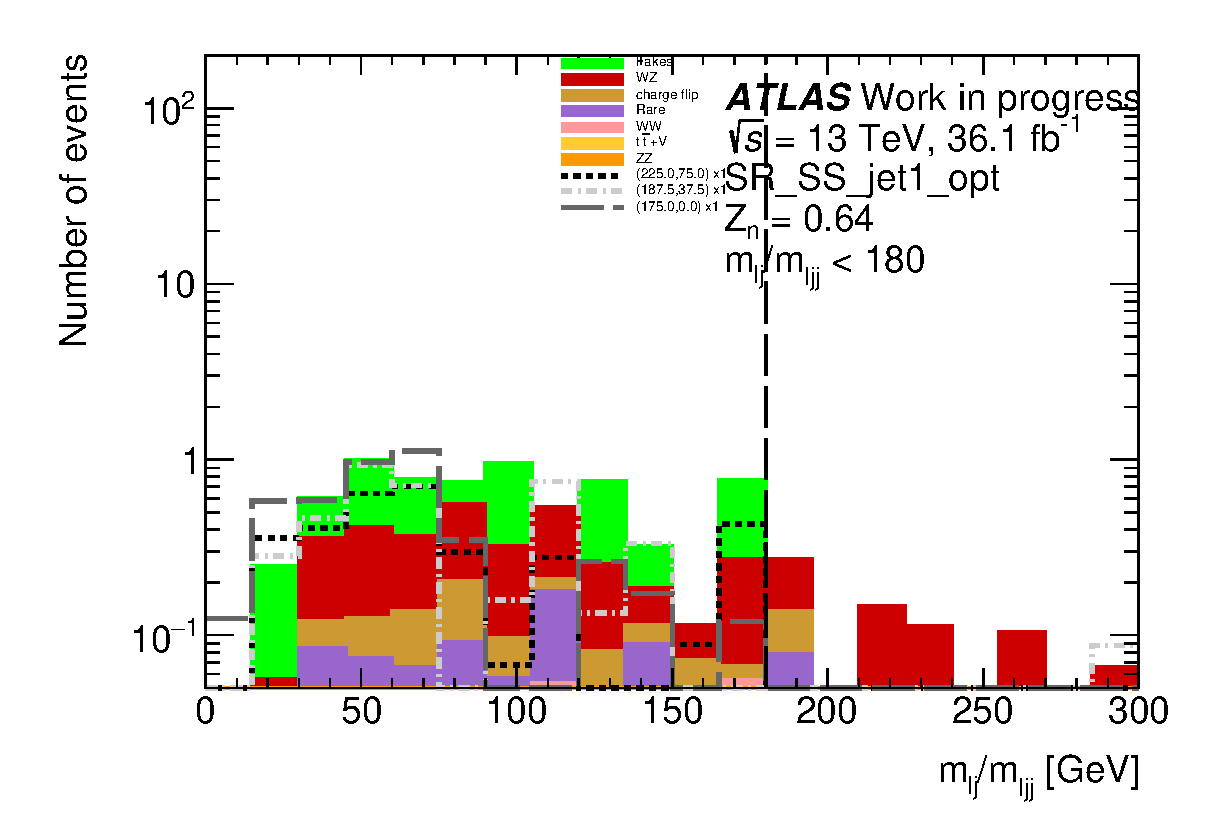
\includegraphics[width=0.45\linewidth]{data/plot/plot_SR/mlj_SR_SS_jet1_opt_0}
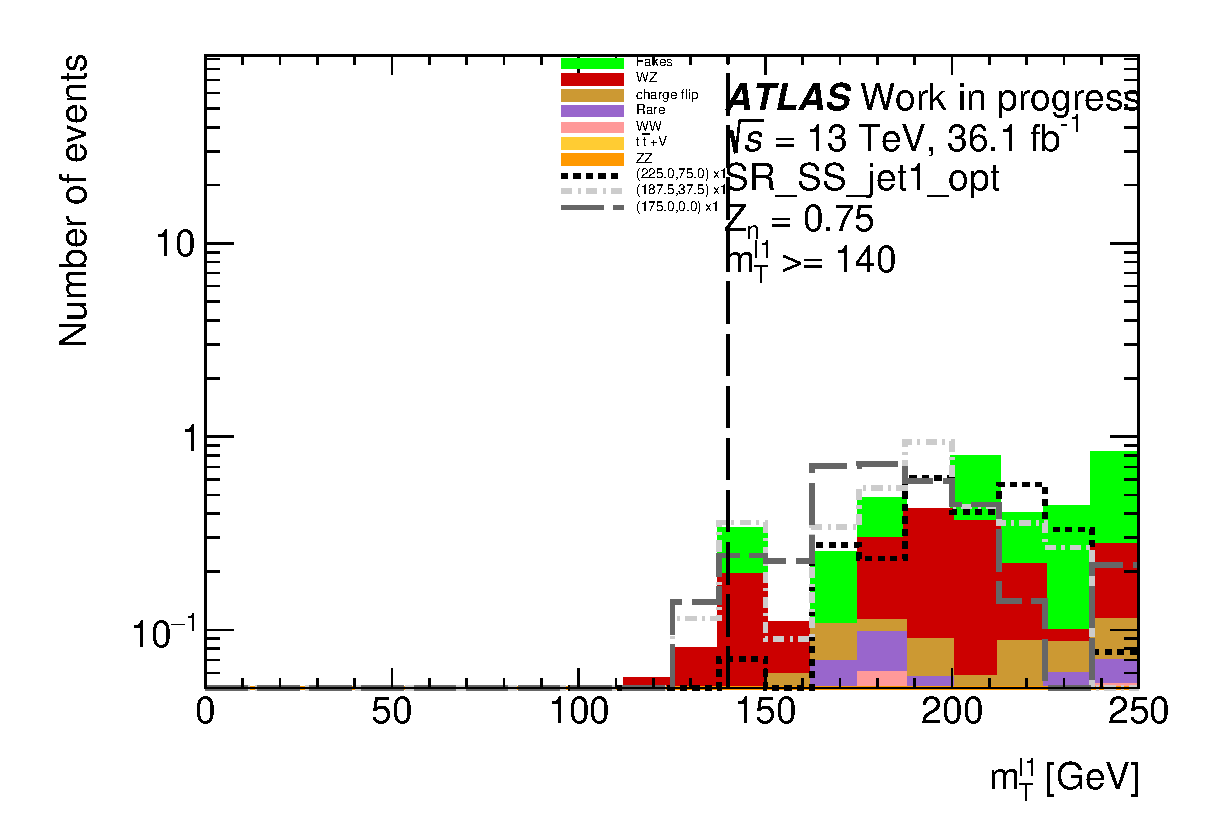
\includegraphics[width=0.45\linewidth]{data/plot/plot_SR/mt1_SR_SS_jet1_opt_0}\\
\caption{The N-1 plots for SRjet1.}
\label{fig:SRjet1_N1}
\end{figure}


\begin{figure}[htpb]
\centering
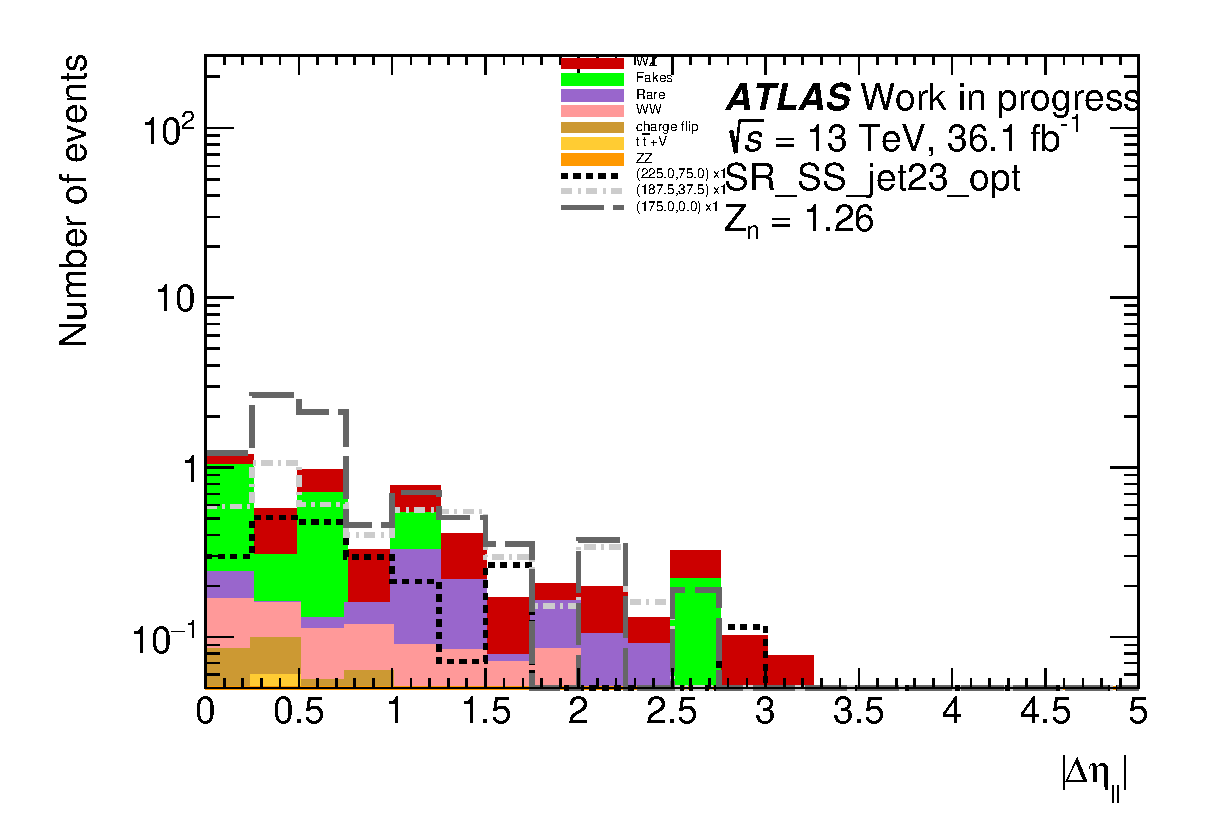
\includegraphics[width=0.45\linewidth]{data/plot/plot_SR/dEta_SR_SS_jet23_opt_0}
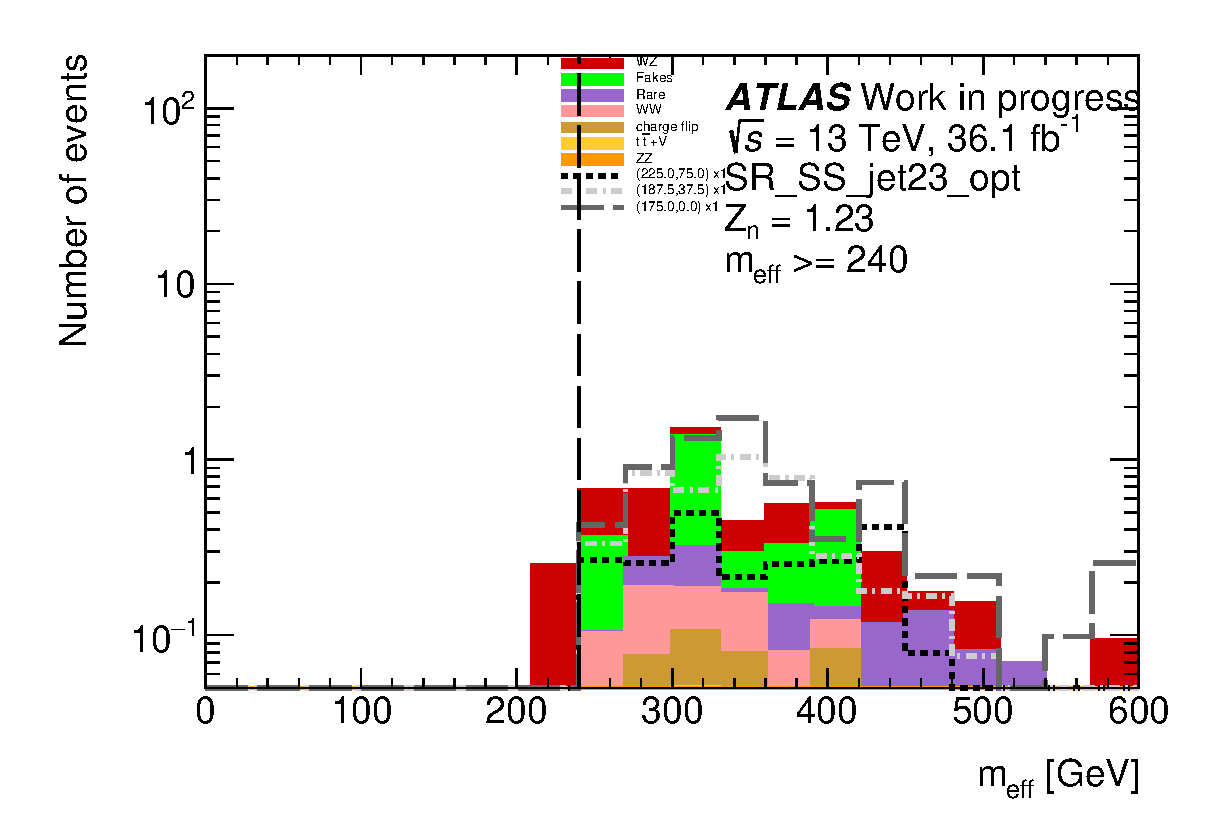
\includegraphics[width=0.45\linewidth]{data/plot/plot_SR/meff_SR_SS_jet23_opt_0}\\
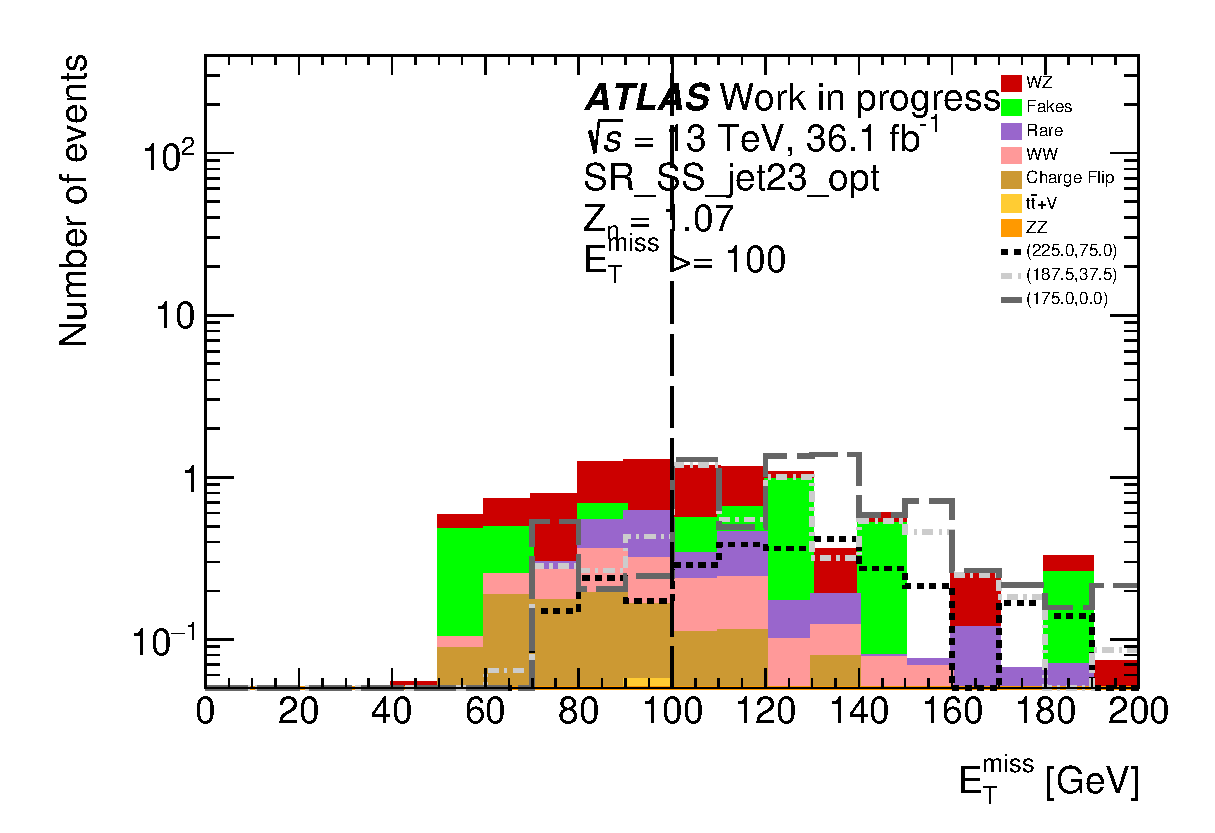
\includegraphics[width=0.45\linewidth]{data/plot/plot_SR/MET_SR_SS_jet23_opt_0}
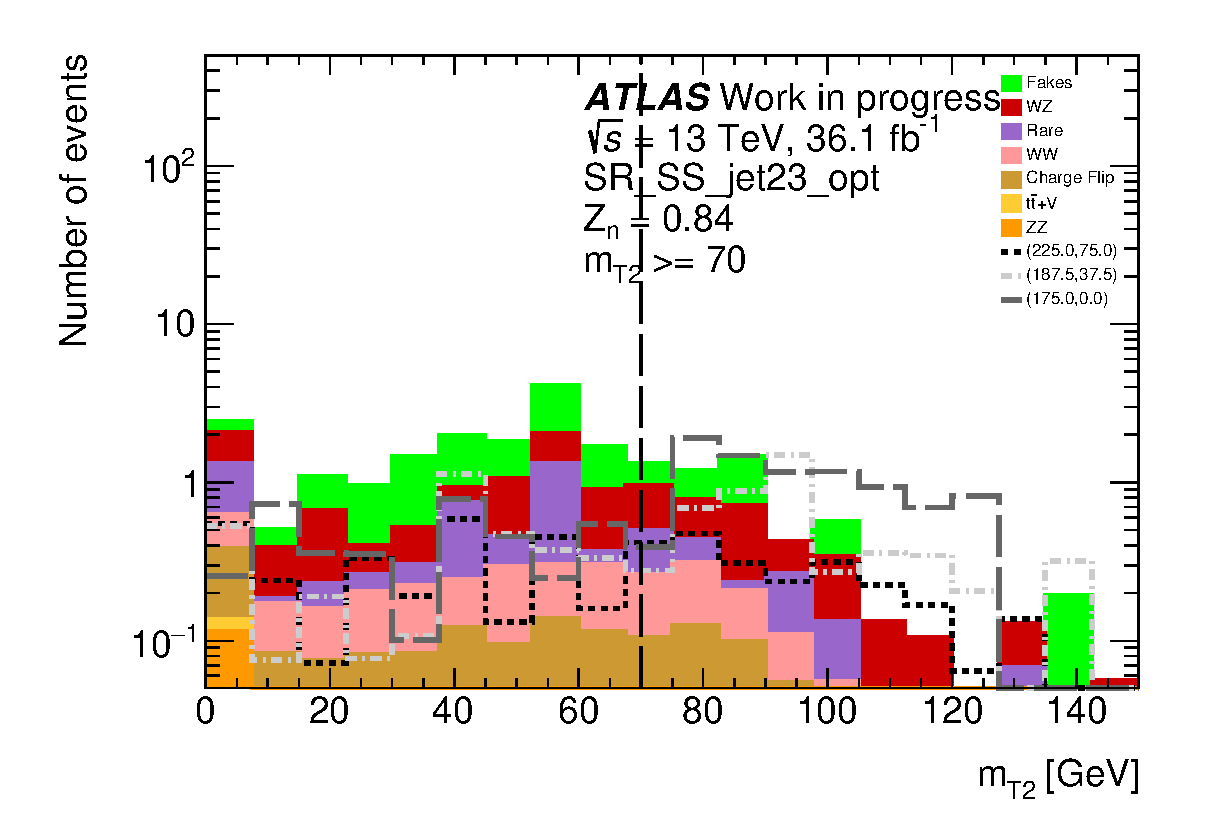
\includegraphics[width=0.45\linewidth]{data/plot/plot_SR/mTtwo_SR_SS_jet23_opt_0}\\
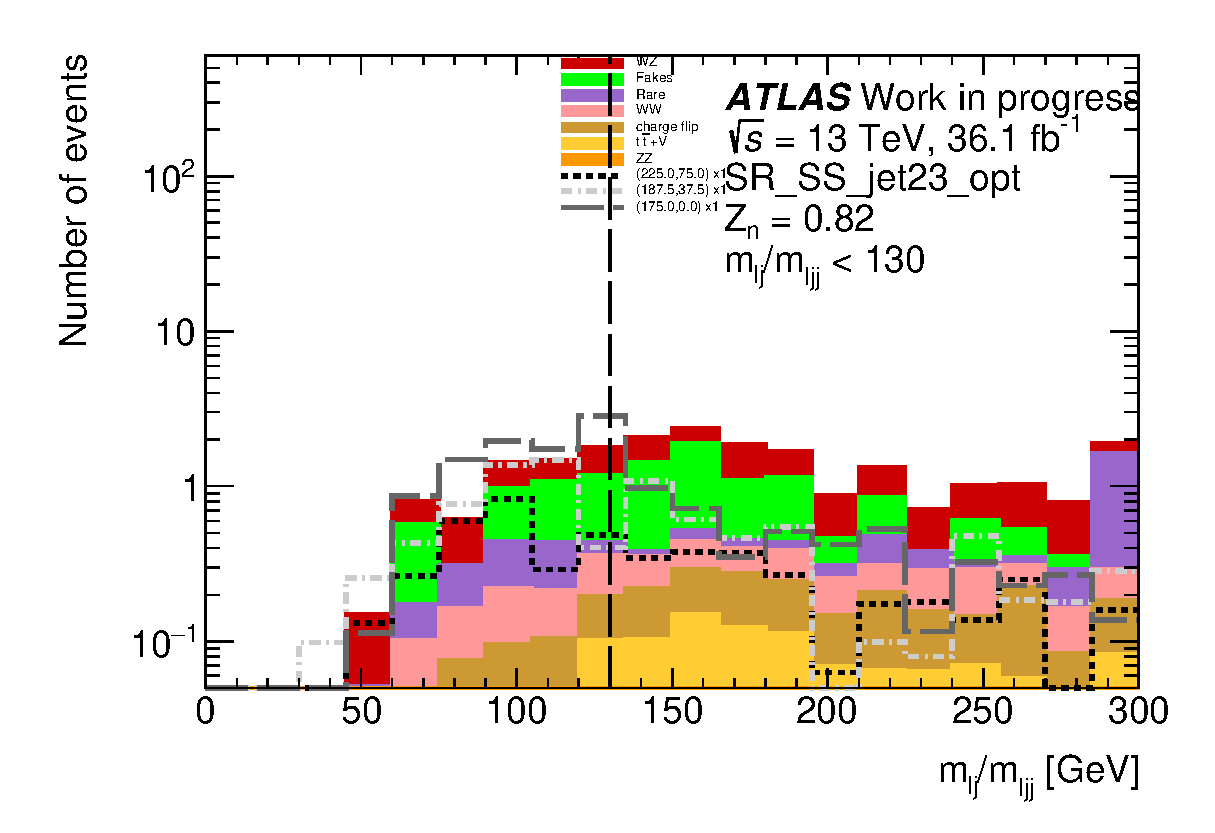
\includegraphics[width=0.45\linewidth]{data/plot/plot_SR/mlj_SR_SS_jet23_opt_0}
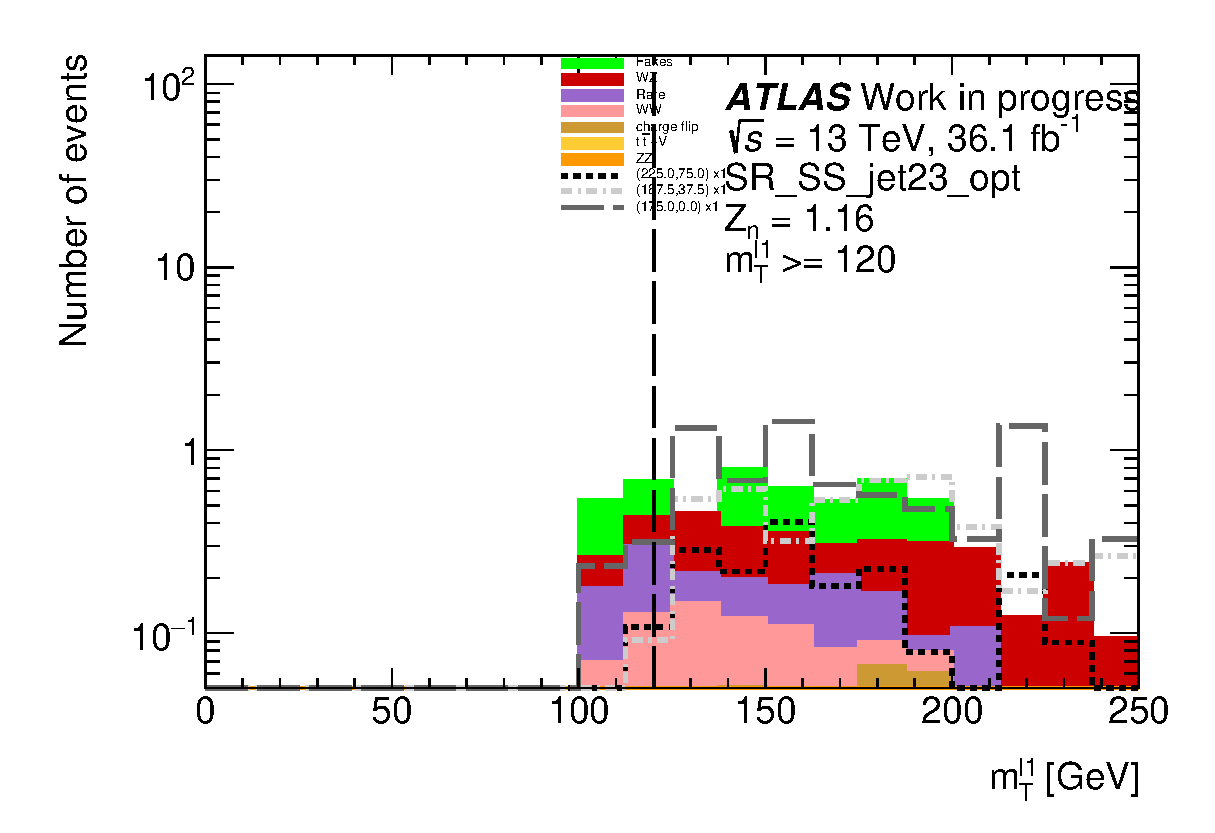
\includegraphics[width=0.45\linewidth]{data/plot/plot_SR/mt1_SR_SS_jet23_opt_0}\\
\caption{The N-1 plots for SRjet23.}
\label{fig:SRjet23_N1}
\end{figure}

The expected combined signal significances for different mass points are shown in figure \ref{fig:SR_expected_limit}.
A flat 25 \% systematic uncertainty are included.
The combined signal significances are calculated by adding the signal significances of the two signal regions in quadrature.
The figure shows considerable signal significances, in particular for the compressed region, where $m_{\tilde{\chi}_1^\pm , \tilde{\chi}_2^0} - m_{\tilde{\chi}_1^0}$ are close to the mass of Higgs boson ($\sim 125$ GeV).

\begin{figure}[htpb]
\centering
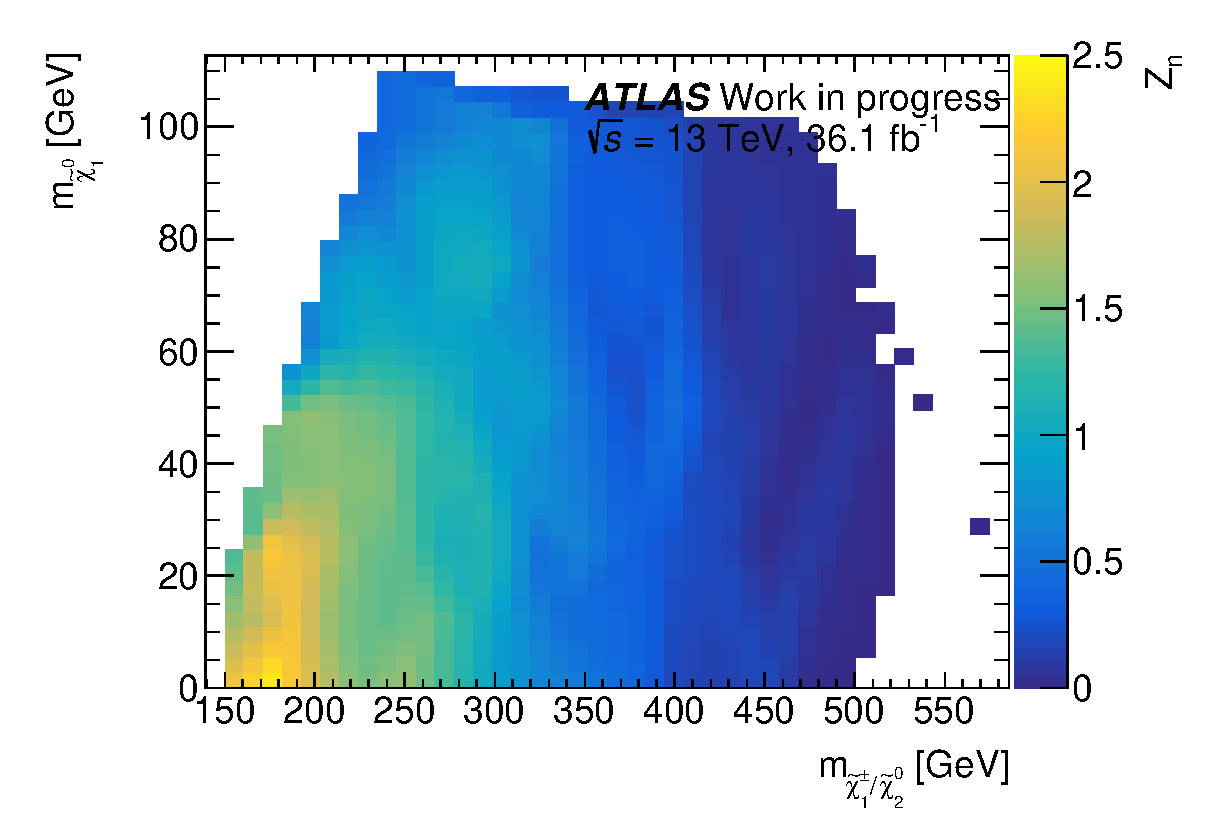
\includegraphics[width=0.5\linewidth]{data/plot/plot_SR/combine_significance_0}
\caption{The expected combined signal significances for different mass points.}
\label{fig:SR_expected_limit}
\end{figure}
